\chapter{Tools}
\emph{Give ordinary people the right tools, and they will design and build the most extraordinary things.\\ -- Neil Gershenfeld}
\newpage
\section{Insert Delay Subroutine}
It is a powerful wizard to generate delay subroutine with user defined delay using any sets of register for a particular operating frequency of 8085 microprocessor.

\begin{figure}[htbp]
	\centering
	\begin{tabular}{c}
		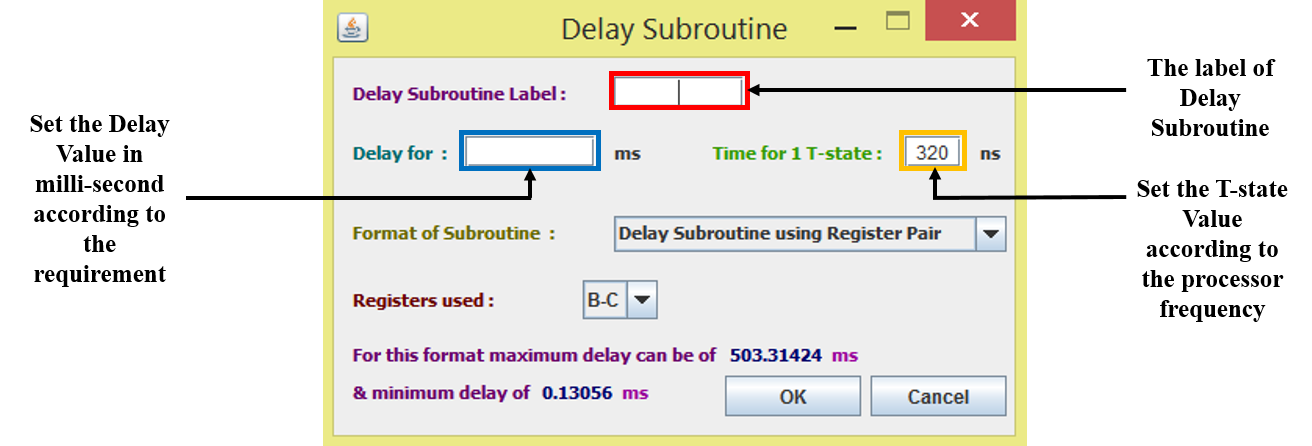
\includegraphics[width=0.8\linewidth]{delay_sub_mark}\\
		(a) Enter the marked boxes, in the order \textbf{Label}, \textbf{T-state} and \textbf{Delay}\\\\
		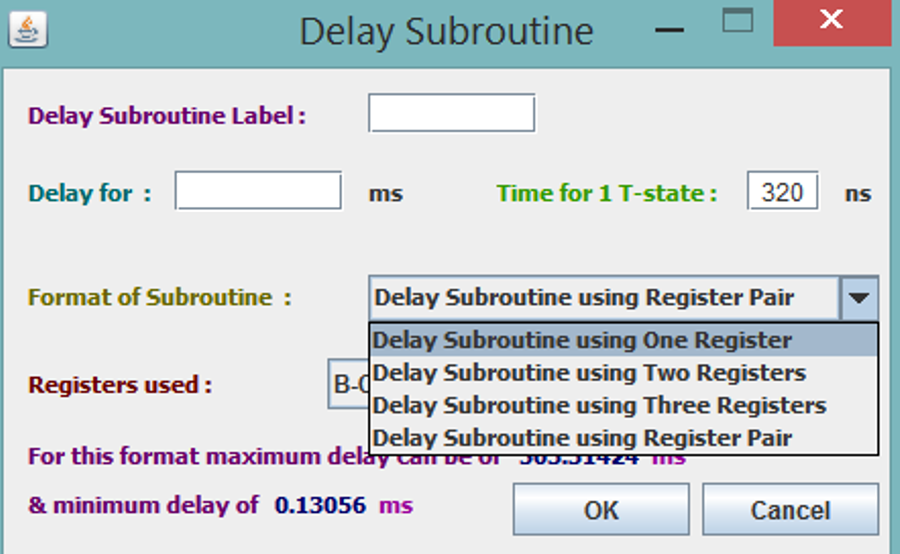
\includegraphics[width=0.5\linewidth]{delay_sub_reg}\\
		(b) Showing the modes supported\\\\
		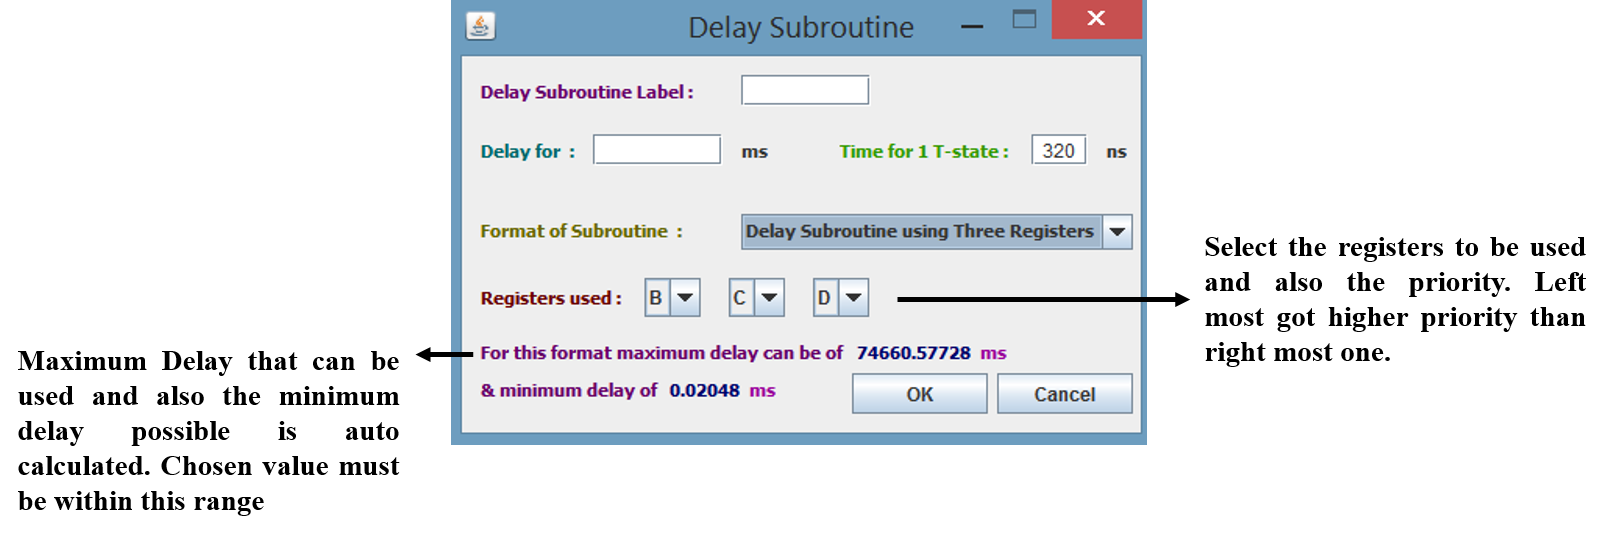
\includegraphics[width=1\linewidth]{delay_sub_reg_choose}\\
		(c)	How to choose the registers
	\end{tabular}
	\caption{The Delay Subroutine dialog box details}
\end{figure}
\newpage
\subsection{Working Example of a delay sub-routine}
\textit{Problem Statement :}
\textbf{\textit{Use 3 registers to generate 10 ms delay in a 8085 having operating frequency of 3.072 MHz.}} \\\\
\textit{Solution::}
The problem is solved using the tool as shown in fig. \ref{fig:delay_sub}.\\
The tool generated values for register $ \mathbf{B = D2~H} $, $\mathbf{ C = 04 ~H}$ and $\mathbf{ D = 01~H }$.\\
After "Run all At a Time" the $ \mathbf{Clock~ Cycle~ Counter = 30697} $\\
The Clock Cycles taken by the delay subroutine is calculated by subtracting the clock cycles taken from the clock cycles of user written code = $\mathbf{ 30697 - 18 - 5 =30674}$.\\
Thus, the time taken by the delay code $= 30674 \times 326 ~ns = \mathbf{9999724~ns} $\\
Error Offset $ = 10,000,000 - 9,999,724 = \mathbf{276 ~ns}$
\begin{figure}[htbp]
	\centering
	\begin{tabular}{cc}
		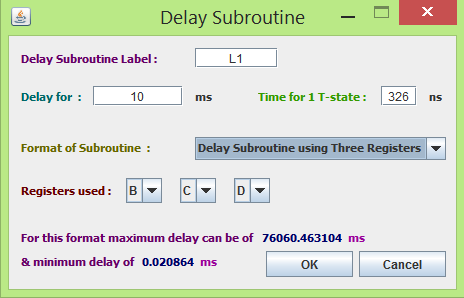
\includegraphics[width=0.5\linewidth]{delay_sub_filled_form} &		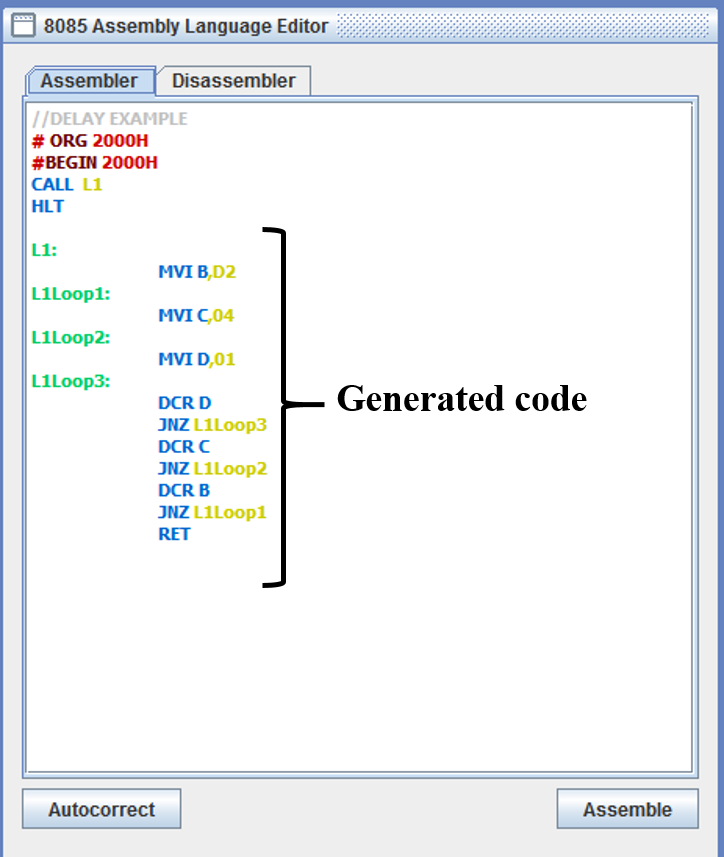
\includegraphics[width=0.5\linewidth]{delay_sub_assembler_editor}\\
		(a) Delay subroutine tool is set to the problem value & (b) The generated code + few user added lines in the top\\\\
		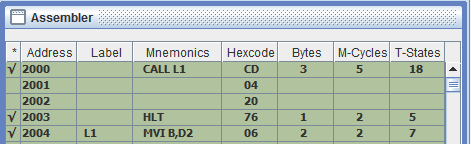
\includegraphics[width=0.5\linewidth]{delay_sub_compiled} & 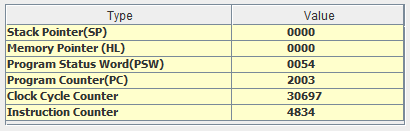
\includegraphics[width=0.5\linewidth]{delay_sub_calc}\\
		(c) Showing the delay of the user added code & (d) Total clock cycles taken by the program after Full Run \\\\
	\end{tabular}
	\caption{Solution of the problem graphically}
	\label{fig:delay_sub}
\end{figure}

\newpage
\section{Interrupt Service Subroutine}
It is a handy way to set memory values at corresponding vector interrupt address.
To invoke the tool select the option `\textbf{Subroutine}' $~ \rightarrow ~$ `\textbf{Interrupt Service Subroutine}'. Fig. \ref{fig:isr_routine} shows the steps to insert Interrupt Service Subroutine to cater to a particular interrupt that refers to a particular call location. In general branch instruction are used in interrupt call location to point to a particular address. 
\begin{figure}[htbp]
	\centering
	{\def\arraystretch{2}
	\begin{tabular}{cc}
			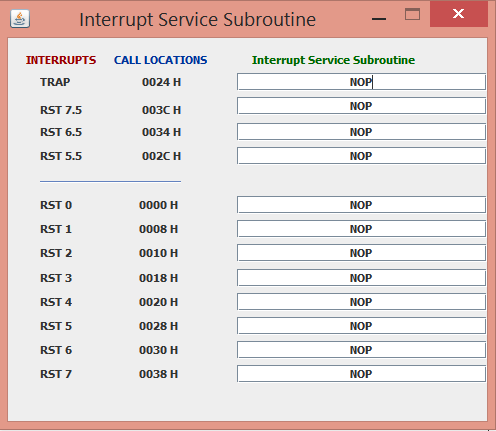
\includegraphics[width=0.5\linewidth]{isr_nop} & 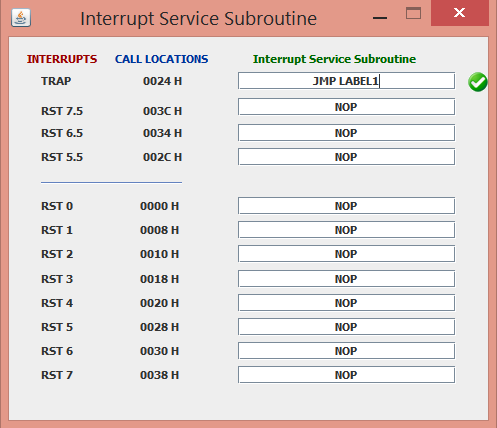
\includegraphics[width=0.5\linewidth]{isr_label}\\
			(a) Showing the entry of TRAP Interrupt & (b) '\textit{Label1}' defined in the \textbf{assembled} code and used in entering\\
			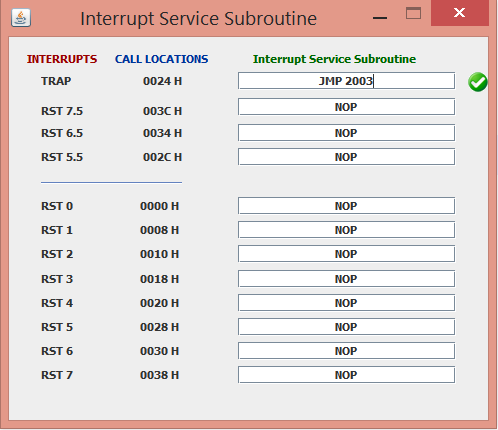
\includegraphics[width=0.5\linewidth]{isr_label_autofill} & 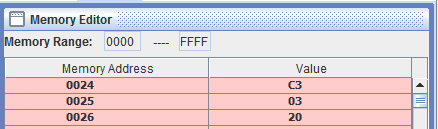
\includegraphics[width=0.5\linewidth]{isr_memory}\\
			(c) On pressing '\textit{Enter}', label is replaced by address & (d) After closing of the window, memory is updated
	\end{tabular}
}
\caption{Procedure to use Interrupt Service Subroutine TOOL}
\label{fig:isr_routine}
\end{figure}

\newpage
\section{Number Conversion Tool}
It is a portable number base conversion tool between Hexadecimal, decimal and binary standards. It allows the developers to use the same software to calculate simple conversion instead of opening a new calculator and also shows all the value in Hexadecimal, decimal and binary format simultaneously

\begin{figure}[htbp]
	\centering
	{\def\arraystretch{2}
		\begin{tabular}{cc}
			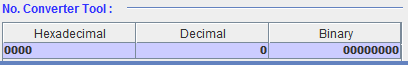
\includegraphics[width=0.5\linewidth]{no_tool} &  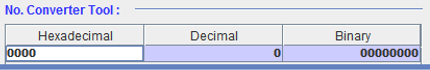
\includegraphics[width=0.5\linewidth]{no_tool_select}\\
			(a) When Unselected & (b) When Hexadecimal text-box is selected\\\\
			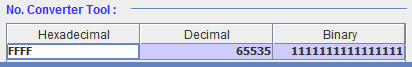
\includegraphics[width=0.5\linewidth]{no_tool_value} &
			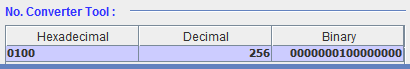
\includegraphics[width=0.5\linewidth]{no_tool_value_dec}\\
			(c) After pressing enter on Hexadecimal text-box & (d) Decimal value of 256 entered\\\\
			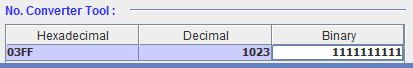
\includegraphics[width=0.5\linewidth]{no_tool_bin} &
			\\
			(e) A 10-bit binary value entered for conversion &
		\end{tabular}	
	}
\caption{Using number conversion tool}
\end{figure}
 
 N.B.: The tool text-boxes correctly support upto "FFFF" Hexadecimal and 8-bit binary full scale value.